\graphicspath{{./figures}}

\section{Specifications}

For specification definition, further calculations should be done. This will allow a list of more detailed, system-level specifications to be created. First, the required communication conditions (link distance, atmospheric effects etc.) are established. Then, power and voltage requirements are expanded on. Finally, system integration is considered.

Typicall balloon satellites reach a maximum height of around 30 km \cite{site-weatherWeatherBalloons}. They rise at a vertical speed of around 20 km/h, and can travel horizontally as fast as 200 km/h when falling. However, a typical distance for such a balloon is 200 km, and therefore an average speed of around 100 km/h will be designed for given the average flight time of longer than 2 hours. At this height, a line-of-sight (LOS) calculator reveals that the horizon is around 600 km, meaning that the antenna could theoretically be placed on sea level. Further, the earth's curvature is found to be negligible at this distance, meaning pythagoras can be used to calculate an LOS distance of 120 km. If LEO heights are to be considered, the curvature of the earth should be taken into account. At a height of 160 km, an LOS distance of 1400 km is required, and at 1000 km, an LOS distance of around 3500 km is required. Since this is much further than the required slant range of 250 km, it will not be designed for initially. However, as mentioned, this could potentially be added as a project expansion.

\begin{figure}[!htb]
    \centering
    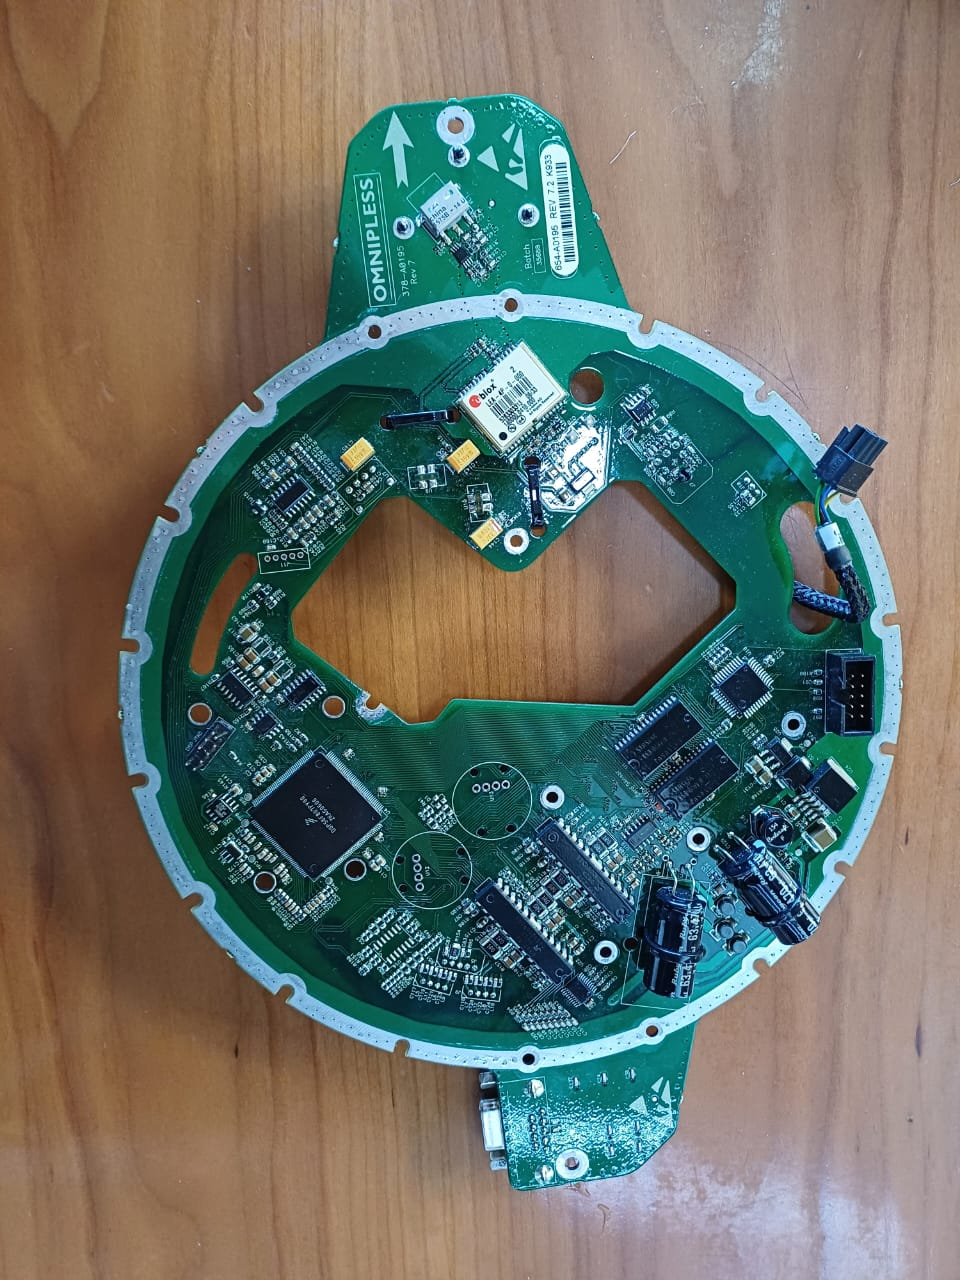
\includegraphics[width=0.4\textwidth, angle=90, origin=c]{gs_existing}
    \caption{Existing Antenna Mount PCB}
    \label{fig:gs_existing}
\end{figure}

The PQ9 standard stipulates a 3V minimum bus voltage. This must therefore be used directly to power the PQ unit circuitry. As mentioned, the PQ unit will be integrated with other \textit{prototype} units into a single PocketQube. Since this is a prototype launch, there is risk of the EPS malfunctioning. Further, a power connection is also needed during development for modularized testing. A simple on-board battery at least matching the standard's voltage, as well as a battery source selector, will therefore be included in the design. This can be used for testing and deployment, however this battery cell could potentially be removed if the EPS is found to meet the \textit{flight-readiness} tests. It should be noted that high-altitude balloons generally remain air-bound for 2-3 hours, where they eventually pop.

Both designed PCBs integrate into the relevant systems. The PQ9 standard clearly defines the dimensions of such a PCB (e.g. 42 mm x 42 mm outer dimensions) and the design should conform to this. The old antenna mount made use of an existing circular PCB with mounting holes and two support "wings", as shown in \ref{fig:gs_existing}. The new GS PCB should conform to this form factor. Lastly, the system should drive the existing stepper motors in the antenna mount.

Further investigation finally leads to the following general system-level specifications:
\begin{enumerate}
    \item The system should be capable of a slant range of 250 km.
    \item The system should operate at a minimum data rate of 9600 baud (at the specified slant range). This data rate is a typical satellite telemetry value as in \cite{paper-deployableAntenna}.
    \item The system should allow for iMet-54 Radiosonde data to be retreived, assuming that the priorietary protocol can be reverse-engineered. This data is GFSK modulated at a pre-selected frequency of between 402 to 405 MHz \cite{datasheet-iMet54}.
    \item A single antenna should be used for both the custom and proprietary protocol on the GS, meaning the custom communication frequency should be as close to 405 MHz as possible (to minimize required antenna bandwidth).
    \item The PQ unit should follow the PQSU standard, stipulating:
    \begin{itemize}
        \item A 42 mm square outer PCB dimension
        \item A 4 mm component height above, and 2 mm below.
        \item A 20-pin header interface, catering for RS-485 and I2C communication, and providing 3.3 V and 5 V power lines.
    \end{itemize}
    \item The PQ unit should include a battery capable of lasting 4 hours at nominal current draw.
    \item The GS should be capable of tracking the balloon at 110 km/h at a distance of 90 km away (10 \% headroom).
    \item The GS PCB connecting to the existing antenna mount, which has a diameter of 20 cm, with equi-spaced mounting holes, wings etc. as in Figure \ref{fig:gs_existing}.
    \item The GS should control two 4218S-15 bipolar stepper motors, which have a maximum current of 0.50 A per phase, each being driven at 24 V.
    \item The GS should provide a USB-C connection to allow a PC to monitor the data in realtime. This should be capable of receiving all data from the link in realtime.
\end{enumerate}